\documentclass[runningheads]{../llncs}

\usepackage{subcaption}
\usepackage{tabularx}
\usepackage{multirow}
\usepackage{booktabs}
\usepackage[export]{adjustbox}
\usepackage{array}
\newcolumntype{L}[1]{>{\raggedright\let\newline\\\arraybackslash\hspace{0pt}}p{#1}}
\newcolumntype{C}[1]{>{\centering\let\newline\\\arraybackslash\hspace{0pt}}p{#1}}
\newcolumntype{R}[1]{>{\raggedleft\let\newline\\\arraybackslash\hspace{0pt}}p{#1}}

% Used for displaying a sample figure. If possible, figure files should
% be included in EPS format.
\usepackage{graphicx}
\graphicspath{{../images/}}

% If you use the hyperref package, please uncomment the following line
% to display URLs in blue roman font according to Springer's eBook style:
\usepackage[colorlinks=true, linkcolor=blue, urlcolor=blue, citecolor=blue, anchorcolor=blue]{hyperref}
\renewcommand\UrlFont{\rmfamily}

\begin{document}

\title{Learning Grasp Evaluation Models Using Synthetic 3D Object-Grasp Representations}

%\titlerunning{Abbreviated paper title}
% If the paper title is too long for the running head, you can set
% an abbreviated paper title here
%
\author{
    Minh Nguyen \inst{1} \and
    Paul G. Pl\"{o}ger \and
    Alex Mitrevski\inst{1} \and
    Maximilian Sch\"{o}bel\inst{1}}
%
\authorrunning{M. Nguyen et al.}
% First names are abbreviated in the running head.
% If there are more than two authors, 'et al.' is used.
%
\institute{Hochschule Bonn-Rhein-Sieg, Grantham-Allee 20, 53757 Sank Augustin, Germany \\
\email{minh.nguyen@smail.h-brs.de}, \email{\{paul.ploeger,aleksandar.mitrevski,maximilian.schoebel\}@h-brs.de}}
%
\maketitle              % typeset the header of the contribution

\begin{abstract}
This project considers the problem of generating data for training grasp evaluation models. Recent advances are reviewed
for four main aspects most relevant to labeled grasp data synthesis, namely feature extraction from perceptual data,
object-grasp representation, grasp evaluation techniques, and data generation techniques. From this review, one may
conclude that while data synthesis for learning a grasp evaluation model is promising, recent approaches are either
limited by difficulties in collecting large-scale human grasp experience, or by the shortcomings of using analytical
metrics to label generated data. Additionally, a completed object grasping pipeline is integrated, from object
detection to grasp pose detection and grasp execution. Two set of experiments are performed on the Toyota Human Support
Robot for two pose estimation methods using this grasping pipeline. The pipeline proves reliable and fast enough for
performing the experiments, being able to execute 20 grasps per object without interruption. While further extension and
optimization are needed, the pipeline enables directly examining and comparing more advanced grasp planning methods in
the future.

\keywords{Grasp learning \and Data synthesis.}
\end{abstract}


\section{Introduction}

\subsection{Motivation}

Robot grasping with multi-fingered robotic hands is a challenging problem, and finding a grasp planning solution which
resembles humans' grasps in dexterity and robustness is still an area of active research.

\subsection{Use Case}

\begin{figure}[h!]
    \centering
    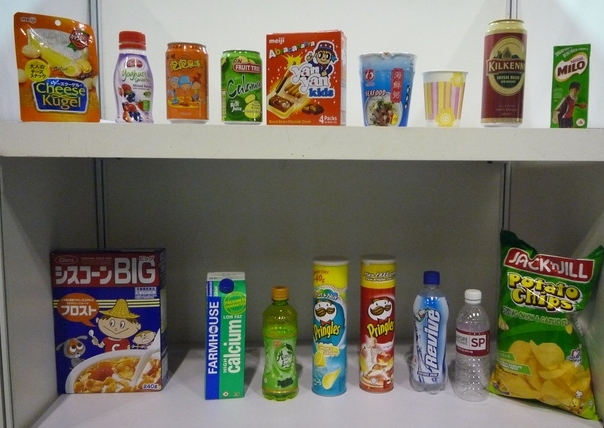
\includegraphics[width=0.5\textwidth]{robocup_typical_objects}
    \caption{Typical objects in the Robocup@Home competition \cite{robocupRulebook2018}.}
    \label{fig:robocup_objects}
\end{figure}

\begin{itemize}
    \item This project focuses on grasping tasks relevant to the Robocup@Home
            \footnote{\url{http://www.robocupathome.org}} competition. These tasks involve objects which can be commonly
            found in a domestic environment, some of which can be seen in figure \ref{fig:robocup_objects}.
    \item The experiments will be conducted on the Human Support Robot (HSR) from Toyota
            \footnote{\url{https://www.toyota-global.com/innovation/partner_robot/robot/}}.
\end{itemize}

\subsection{Overview of robotic grasping research}

\begin{figure}[h!]
    \centering
    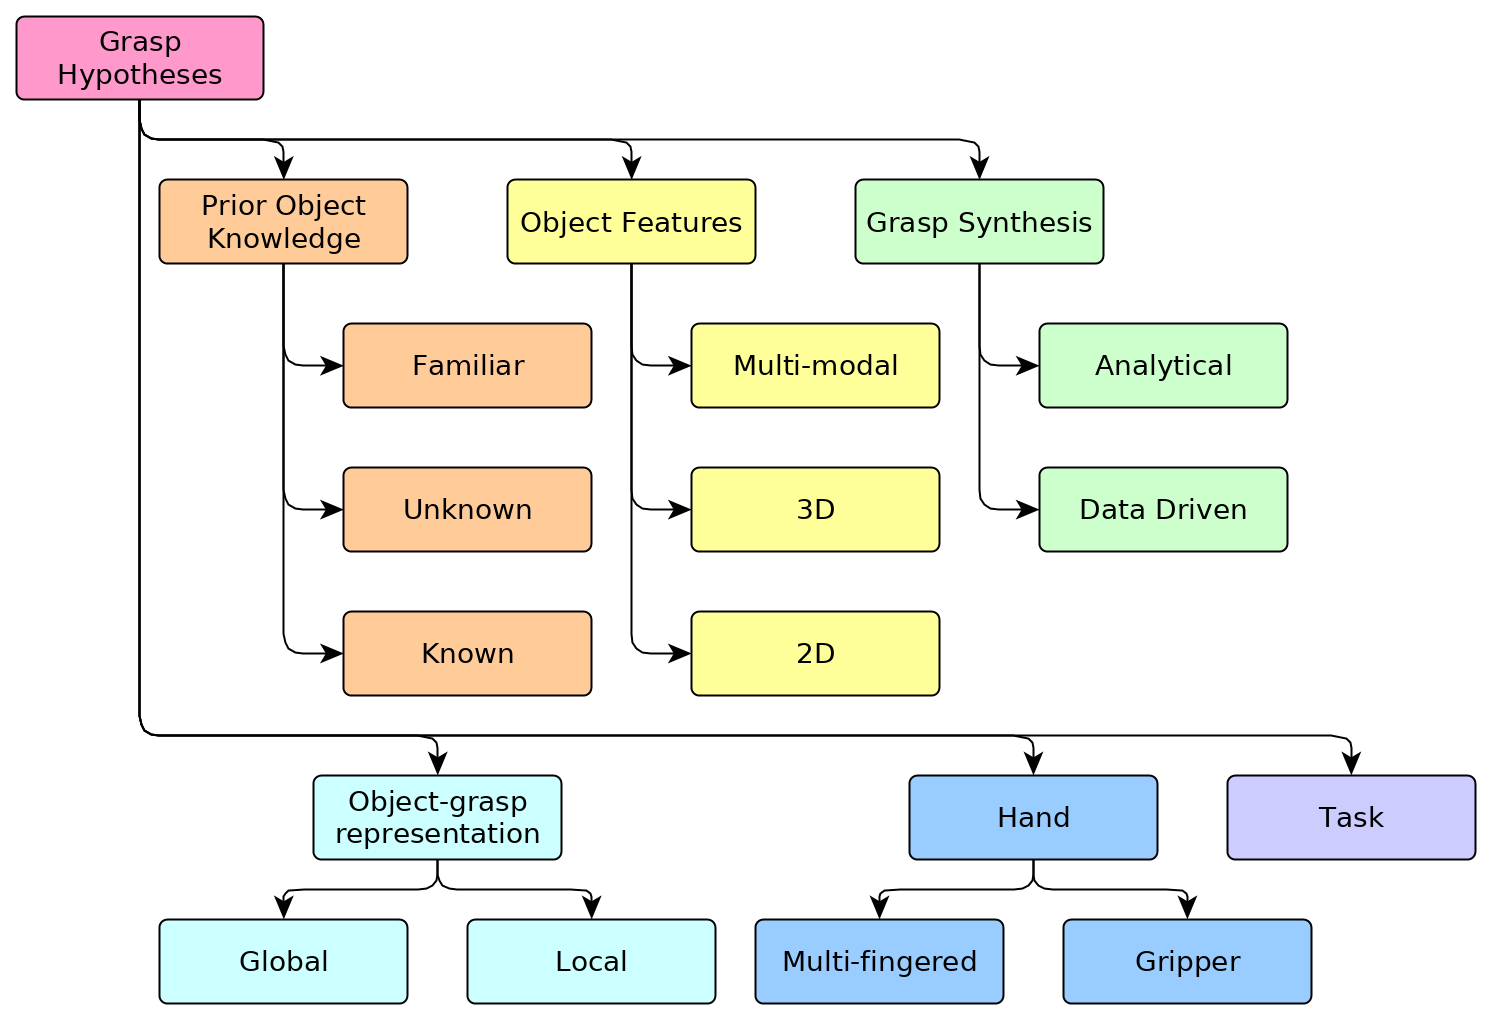
\includegraphics[width=\textwidth]{bohg14-grasp_synthesis_mind_map}
    \caption{Aspects which may influence generation of grasp hypotheses \cite{Bohg2014}.}
    \label{fig:grasp_synthesis_mind_map}
\end{figure}

Sahbani et al. \cite{Sahbani2012} classify grasp synthesis into analytical and empirical approaches:

\begin{itemize}
    \item Analytical methods consider mechanical properties of the contact points between the gripper's fingers and an
    object \cite{Roa2015,Sahbani2012,Shimoga1996}: disturbance resistance, dexterity, equilibrium and stability.
    \item Empirical methods rely on some form
of grasp experience to synthesize candidates. Bohg et al. \cite{Bohg2014}
    organize them based on how much information is assumed about the object: whether they are known, familiar or
    completely unknown to the robot.
\end{itemize}

\section{State of the Art}

\subsection{Feature extraction from perceptual data for grasping}

\begin{itemize}
    \item Several approaches Convolutional Neural Networks (CNN) to combine depth and RGB features
            \cite{Eitel2015,Gupta2014RGBDFeatures,Porzi2017}
    \item Some approaches predict regions occluded in the RGB-D point clouds \cite{Qi2016,Su2015} or reconstruct objects
            from the incomplete view of a single RGB-D camera \cite{Bohg2011MindTheGap,Varley2017}.
\end{itemize}

\subsection{Object-grasp representation}

\begin{itemize}
    \item Based on global features: can use CNN on RGB-D image of object \cite{mahler2017} or eigengrasps
            \cite{Ciocarlie2009,Goldfeder2011}.
    \item Based on local features: extract features from the rectangle/cuboid regions corresponding to a two-fingered
            gripper \cite{Detry2012,lenz2015,jiang2011}, or local template grids at points of contact
            \cite{Kappler2015}.
\end{itemize}

\subsection{Grasp evaluation}

\begin{table}[h!]
\scriptsize
\def\arraystretch{1.2}
\begin{tabularx}{\linewidth}{L{0.05\linewidth}C{0.39\linewidth}L{0.28\linewidth}L{0.28\linewidth}}
    Method & Object-grasp\linebreak representation & Feature extraction \& learning model & Data generation \\
    \toprule
    \cite{jiang2011}    & 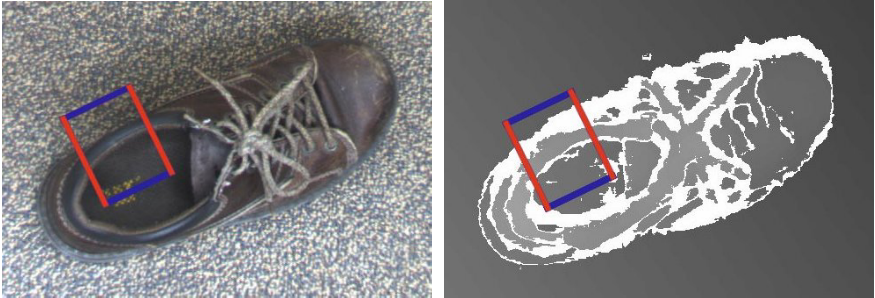
\includegraphics[scale=0.09,valign=t]{jiang_et_al-2011-grasp_representation}
    & Histogram of hand-crafted filters; \linebreak Model: SVM.
    & Rectangles manually \linebreak annotated. \\
    \cite{lenz2015}     & 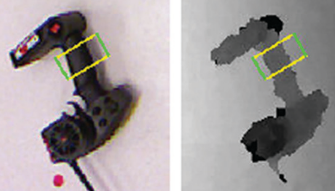
\includegraphics[scale=0.16,valign=t]{lenz_et_al-2015-grasp_representation}
    & Auto-encoders to initialize weights, structured regularization to combine depth
    and RGB data; \linebreak Model: MLP.
    & Extension of the \linebreak dataset from \cite{jiang2011} \linebreak (above).\\
    \cite{Kappler2015}  &
    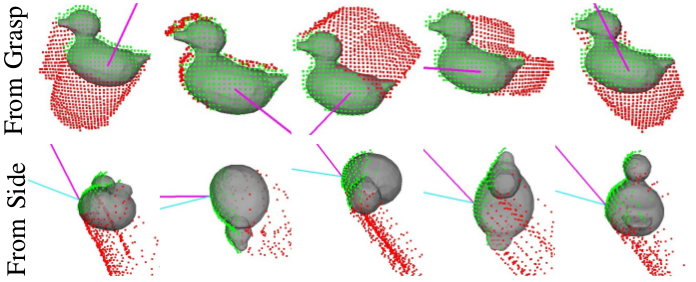
\includegraphics[scale=0.16,valign=t]{kappler_et_al-2015-fig8-local_shape_diff_viewpoints}
    & RGB rendering of ``template grids''; \linebreak Model: LeNet CNN
    & Quality of grasps are \linebreak calculated in simulation \linebreak for object
    meshes, \linebreak verified via crow-sourcing. \\
    \cite{Gualtieri2016}& 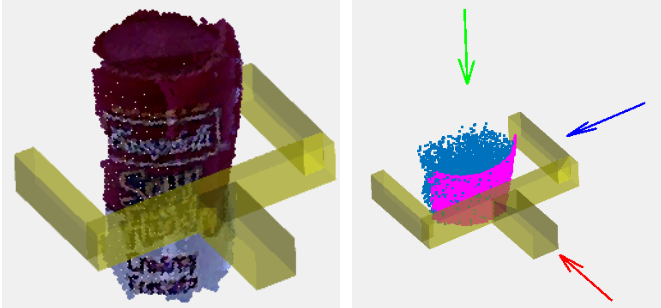
\includegraphics[scale=0.1,valign=t]{Gualtieri_et_al-2016-grasp_representation}
    & Filters of cuboid regions projected onto 3 orthogonal planes, creating 15 channels;
    \linebreak Model: LeNet CNN.
    & Quality of grasps are \linebreak calculated for object \linebreak meshes using
    force-closure \\
    \cite{mahler2017}   & 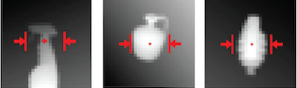
\includegraphics[scale=0.22,valign=t]{mahler_et_al-2017-grasp_representation}
    & Depth images cropped and aligned to gripper; \linebreak Model: CNN combined
    with single-layer NN.
    & Quality of grasps are \linebreak calculated for object \linebreak meshes using a
    variant of $ \epsilon $-metric from \cite{WeiszAllen2012} \\
    \bottomrule
\end{tabularx}
\caption{\scriptsize Five recent empirical approaches to grasp quality prediction}
\label{table:grasp_approaches}
\end{table}

\begin{itemize}
    \item Analytical grasp metrics: focus on form/force closure properties, generally via analyzing the grasp matrix
            $ G $, the force wrench space (FCS), the grasp wrench space (GSP), or the hand-object Jacobian $ J $.
    \item Analytical metrics can be extended to consider task affordance via limiting the analysis only to movements 
            relevant to performing a specific task.
    \item Learning to predict grasp quality: table \ref{table:grasp_approaches} summarize the most prominent approaches.
\end{itemize}

\subsection{Generating data for grasp success prediction}
\begin{itemize}
    \item Data synthesis for robot grasping
    \item Data augmentation
\end{itemize}

\section{Methodology}

\subsection{Object detection}

\begin{figure}[h!]
    \centering
    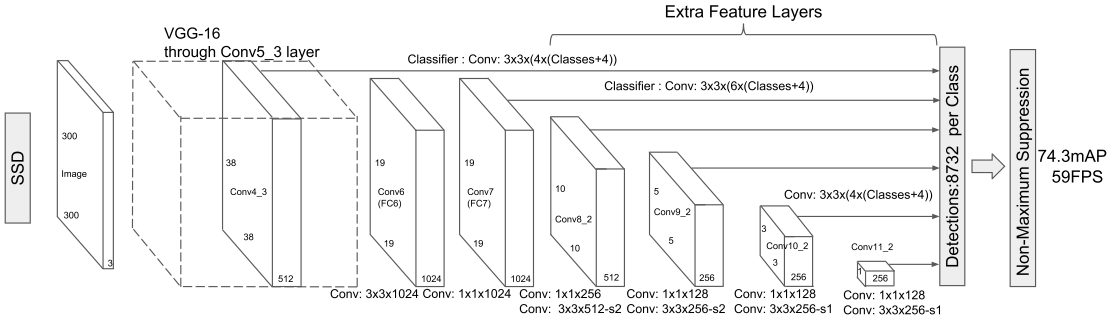
\includegraphics[width=\textwidth]{liu_et_al-2016-ssd_arch}
    \caption{SSD architecture \cite{Liu2016SSD}.}
    \label{fig:ssd_arch}
\end{figure}

Integrate Single-Shot Multibox Detector (SSD) for object detection (figure \ref{fig:ssd_arch})

\subsection{Pose estimation and grasping}
\subsubsection{Baseline method}
\begin{figure}[h!]
    \centering
    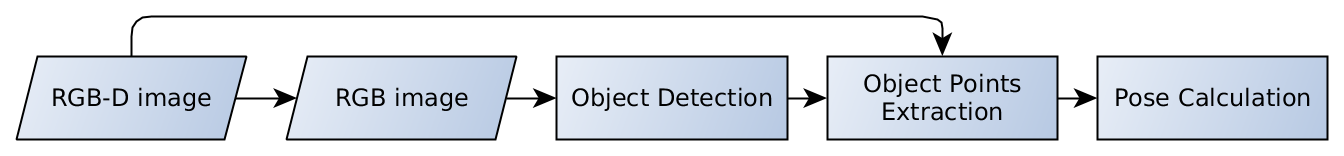
\includegraphics[width=\textwidth]{grasp_plan_pose_estimation}
    \caption{Flowchart of the baseline method for grasp experiments.}
    \label{fig:grasp_plan_baseline}
\end{figure}

\begin{itemize}
    \item assume the grasp approach to be along the $ x $-axis of the robot
    \item extract object points using image detection result
    \item estimate object positions in the \texttt{base\_link} coordinate frame
    \item estimated $ y $- and $ z $-coordinates are mean of the object points
    \item estimated $ x $-coordinate is either the minimum or mean of the object points
\end{itemize}

\subsubsection{Grasp Quality CNN (GQCNN)}
\begin{figure}[h!]
    \centering
    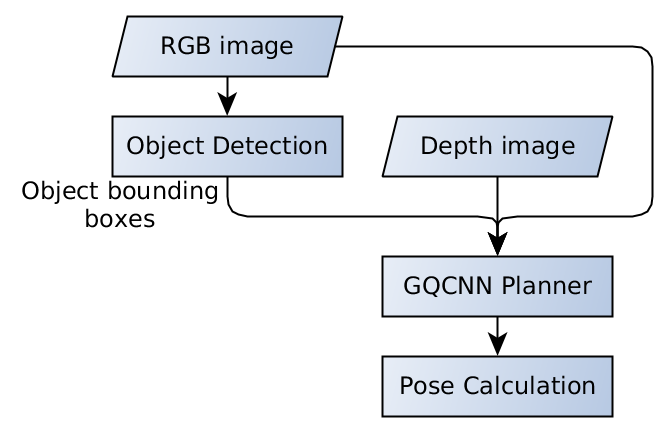
\includegraphics[width=0.5\textwidth]{grasp_plan_gqcnn}
    \caption{Flowchart of the integrated GQCNN grasp planner \cite{mahler2017}.}
    \label{fig:grasp_plan_gqcnn}
\end{figure}

\begin{itemize}
    \item GQCNN model \cite{mahler2017} is trained on Dex-Net 2.0 dataset to predict grasp robustness,
    \item In the original setup, the grasp is assumed to be from above and perpendicular with the table,
    \item Grasp approach vector is assumed to align with camera axis,
    \item Not reliable enough for performing grasp experiments.
\end{itemize}

\begin{figure}[h!]
    \centering
    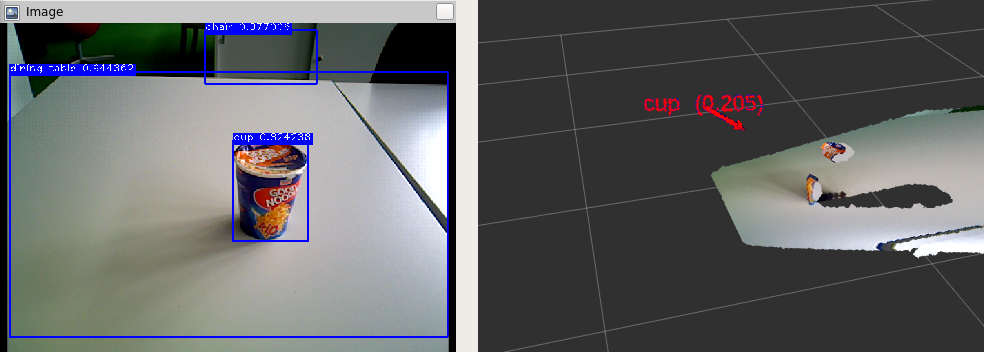
\includegraphics[width=0.9\textwidth]{grasp_gqcnn_result}
    \caption{A successful GQCNN grasp plan. Arrow and number on the right indicate grasp pose and quality returned from
             the GQCNN planner.}
    \label{fig:gqcnn_result}
\end{figure}

\section{Experiments}

\subsection{Experimental Setup}

\begin{itemize}
    \item Two sets of experiments are performed for the variances of the baseline method described in slide
    \item Before each grasp, the robot is moved to a marked position facing the dining table.
    \item Objects further than 90cm in $ x $-axis and lower than 75cm in $ z $-axis are ignored.
    \item We use the SSD model pre-trained on the COCO dataset.
    \item Arm collisions and object slips are counted as failures.
    \item Only one of the objects in figure \ref{fig:objects} is grasped at a time.
\end{itemize}

\begin{figure}[h!]
    \centering
    \begin{subfigure}[t]{0.23\textwidth}
        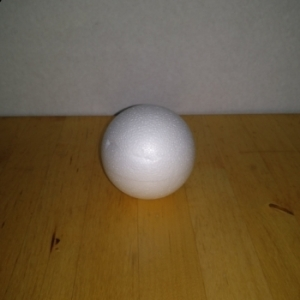
\includegraphics[width=\textwidth]{object_ball}
        \caption{\scriptsize Styrofoam ball}
        \label{fig:object_ball}
    \end{subfigure}
    ~
    \begin{subfigure}[t]{0.23\textwidth}
        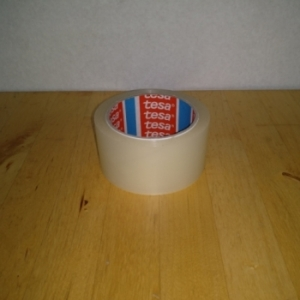
\includegraphics[width=\textwidth]{object_duct_tape}
        \caption{\scriptsize Duct tape}
        \label{fig:object_duct_tape}
    \end{subfigure}
    ~
    \begin{subfigure}[t]{0.23\textwidth}
        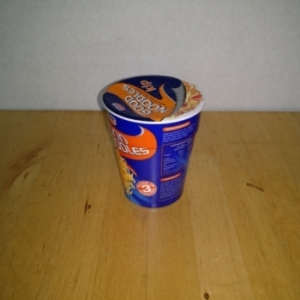
\includegraphics[width=\textwidth]{object_noodle_box}
        \caption{\scriptsize Noodles box}
        \label{fig:object_noodle_box}
    \end{subfigure}
    ~
    \begin{subfigure}[t]{0.23\textwidth}
        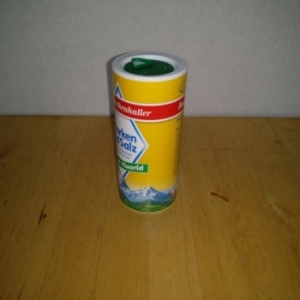
\includegraphics[width=\textwidth]{object_salt}
        \caption{\scriptsize Salt container}
        \label{fig:object_salt}
    \end{subfigure}
    \caption{Objects selected for the experiments.}\label{fig:objects}
\end{figure}

\subsection{Results}

\begin{table}[h!]
    \centering
    \begin{tabularx}{\textwidth}{L{0.3\textwidth}C{0.16\textwidth}C{0.16\textwidth}C{0.16\textwidth}C{0.16\textwidth}}
        \cmidrule[0.08em](){1-5}
        \multirow{2}{*}{Object} & \multicolumn{2}{c}{Mean $ x $} & \multicolumn{2}{c}{Minimum $ x $}    \\
        \cmidrule[0.08em](){2-5}
        & Success   & Failure               & Success   & Failure               \\
        \cmidrule[0.08em](){1-5}
        Salt                    & 17        & 3                     & 16        & 4                     \\
        Ball                    & 8         & 12                    & 15        & 5                     \\
        Noodle box              & 16        & 4                     & 12        & 8                     \\
        Duct tape               & 7         & 13                    & 13        & 7                     \\
        \cmidrule[0.08em](){1-5}
    \end{tabularx}
    \caption{Results of the grasp experiments. On the left are results from using the mean $ x $ coordinates for
        estimating the grasp pose, and on the right are results from using the min coordinates along the
        $ x $-axis.}
    \label{table:grasp_exp_result}
\end{table}

\section{Conclusion}
\subsection{Contributions}
The first contribution of this work is a detailed review of recent advances in aspects most relevant to generating data
for training a grasp evaluation models, namely feature extraction from perceptual data, object-grasp representation,
grasp evaluation metrics, and data generation techniques. Additionally, five recent, prominent approaches to data
synthesis for grasp evaluation are examined, and their solutions for each of the four aspects mentioned above are
summarized in table \ref{table:grasp_approaches}.

The second contribution of this project is the implementation of a full grasping pipeline, from perceiving objects to
grasp execution, in collaboration with another Research and Development project by Padalkar \cite{Padalkar2018}. Two
pose estimation methods are implemented, serving as baselines for experimenting and comparing with more advanced grasp
planning techniques.

The review of recent approaches to grasp data synthesis demonstrates their limitations either in dataset size or by
using theoretical approaches to generate data labels, suggesting possible extensions and improvements with larger human
grasp experience database \cite{Saudabayev2018} or more advanced feature extraction methods \cite{Varley2017}.

\subsection{Future work}

\begin{itemize}
    \item Grasp execution can be extended for grasping from multiple directions.
    \item SSD model for detection can be fine-tuned for RoboCup objects.
    \item Grasp pipeline should be tested on the Care-o-bot.
    \item More advanced method can be implemented to find better pose estimates using the object points.
    \item Surface normal can be calculated for a better approach vector estimate.
    \item Approaches in table \ref{table:grasp_approaches} can be integrated and extended with new human grasp
    database \cite{Saudabayev2018}.
    \item Techniques introducing task awareness into data generation and labeling can also be examined.
\end{itemize}

%
\bibliographystyle{../splncs04}
\bibliography{../RnD}
%

\end{document}
